% Template for ICASSP-2018 paper; to be used with:
%          spconf.sty  - ICASSP/ICIP LaTeX style file, and
%          IEEEbib.bst - IEEE bibliography style file.
% --------------------------------------------------------------------------
\documentclass{article}
  \usepackage{spconf,amsmath,graphicx,amssymb}
  
  % Example definitions.
  % --------------------
  \def\x{{\mathbf x}}
  \def\L{{\cal L}}
  
  % Title.
  % ------
  \title{Quantifying Graphical Password Strength by neural networks}
  %
  % Single address.
  % ---------------
  % \name{Author(s) Name(s)}
  % \address{Author Affiliation(s)}
  %
  % For example:
  % ------------
  %\address{School\\
  %	Department\\
  %	Address}
  %
  % Two addresses (uncomment and modify for two-address case).
  % ----------------------------------------------------------
  \twoauthors
   {Yushuo Guan, Yuanxing Zhang, Kaigui Bian}
    {Peking University\\
    School of Electrical Engineering and Computer Sciences\\
    China, 100871}
   {Lin Chen}
    {Yale University\\
    Department of Electrical Engineering\\
    USA}
  %
  \newtheorem{definition}{Definition}
  \begin{document}
  %\ninept
  %
  \maketitle
  %
  \begin{abstract}
  Nowadays, graphical passwords are broadly implemented in mobile devices. The diversity of images and sketches 
  in graphical passwords greatly increases theoretical complexity, but may not reduce the risk of 
  shoulder-surfing attacks. Especially with the development of neural networks, shoulder-surfing attacks are 
  simplified so that graphical passwords are under more risks than ever. In this paper, we proposed a method 
  to quantify graphical password strength against NN enabled shoulder-surfing attacks. To our best knowledge, 
  it is the first work in related fields.
  \end{abstract}
  %
  \begin{keywords}
  graphical passwords, shoulder-surfing attacks, quantitative analysis
  \end{keywords}
  %
  \section{Introduction}
  \label{sec:intro}
  
  In today of the network information times, people are increasingly using graphical passwords
  to login their online accounts and access personal information(e.g., visit Facebook or Twitter). 
  Graphical passwords are knowledge-based passwords, motivated by the idea that correlates images 
  or sketches with the shared secret \cite{DBLP:journals/csur/BiddleCO12}. 
  The simplest applications of graphical passwords are Personal Identification Number (PIN) 
  and text passwords, directly using numbers and characters to form passwords. More advanced passwords 
  add complex symbols into their systems, like human faces or pictures \cite{Passfaces}, 
  \cite{DBLP:conf/uss/JermynMMRR99}, \cite{DBLP:conf/soups/WiedenbeckWBBM05}.
  
  The diversity of pictures improves the theoretical complexity of graphical passwords, but 
  may not reduce the risk of shoulder-surfing attacks. Shoulder-surfing attacks, also known as peeping attacks, 
  are defined as attacks during which adversaries can observe all actions of humans on input terminals and 
  interactions between humans (provers) and computers (verifiers) \cite{DBLP:journals/iacr/LiS05}. Attackers may utilize direct observation or 
  high-resolution cameras to record passwords. The theoretical complexity of password schemes will decrease 
  quickly after successive shoulder surfing attacks. For example, the remaining theoretical complexity of text 
  password will decrease to $O(1)$ after attackers recorded the whole authentication process.
  
  For many advanced graphical passwords, it is largely insufficient for attackers to crack the password merely 
  with the records of users, since there might be mappings between the input and password. There is no 
  standardized mechanism to find the mappings in the past, so the efficiency of shoulder-surfing attacks fluctuated 
  wildly between different attackers. However, the revolution in neural network (NN) simplified 
  shoulder-surfing attacks, an advantage of NNs is that they do not need hand-crafted features and can be 
  applied directly to “raw” observations, so NNs are helpful to automatically learn the mappings between the 
  input and password. 
  
  More importantly, NN makes it possible for researchers to quantify the strength of passwords against 
  shoulder-surfing attacks. On account of wild fluctuations on the efficiency between different attackers, 
  traditional analysis can only make qualitative analysis on password strength against shoulder-surfing attacks. 
  Usually they made a certain questionaire in advance and collected feedback from a group of participants, which 
  is coarse-grained and inaccurate. NN makes the attack model standardized and provides researchers with an opportunity 
  to quantify graphical passwords strength against shoulder-surfing attacks. 
  
  In this paper, we proposed a standardized method to quantify the password strength. We first revised basic 
  definitions with respect to the password architecture and proposed a indicator to measure password strength against 
  shoulder surfing attacks. We then built up different NN models for graphical passwords with 
  single or multiple bits of input. We quantified four representative graphical password schemes in the experiments and verified 
  the rationality of the indicator. Other researchers may build upon this approach to analyze future systems.
  
  To our best knowledge, our work is the first to quantify the password strength against shoulder-surfing 
  attacks. Recent work has focused on the invention of shoulder-surfing resistant authentication. Some of them 
  proposed theoretical principles to frustrate shoulder-surfing attacks. Shujun Li \cite{DBLP:journals/iacr/LiS05} 
  mentioned three basic principles: time-variant responses, uncertainty and balance. Nicholas Hopper 
  \cite{Hopper:2001:SHI:647097.717000} introduced formal definitions of completeness, soundness and human 
  excutability. Extension works proposed specialized solutions in different fields. 
  \cite{DBLPHK17} and \cite{DBLPJW17} made shoulder-surfing resistant schemes 
  for augmented reality, \cite{DBLP:journals/mta/LuoY16} and \cite{DBLPOF15} presented 
  specific schemes for smartphones to prevent shoulder-surfing attacks. All these works were verified by a small 
  number of volunteers, which is less convincing than a quantitative analysis.
  
  \section{Definitions and system architecture}
  \label{sec:preliminaries}
  In this section, we first presented basic definitions with respect to an authentication, and then introduced the 
  architecture in the graphical password systems.
  \subsection{Basic Definitions}
  The most fundamental definitions in the authentication process are authentication challenges and answers. To 
  login, users have to enter an answer into the system (like "123456") based on a given challenge (like "Please 
  enter your password.").
  \begin{definition}
    \textbf{Authentication Challenge $\vec c$ and Challenge Space $\mathbb{C}$}. $\vec c = [x_1, x_2,...,x_M]$, 
    wich contains $M$-bit messages for computers (verifiers) to distinguish users from malicious impersonators. 
    Challenge space contains all possible authentication challenges that one graphical password system can 
    provide. $|\mathbb{C}| = \prod\limits_{i=1}^{M}|S_x^i|$, where $S_x^i$ contains all possible options for 
    the $i$-th bit message of an authentication challenge.
  \end{definition}
  \begin{definition}
    \textbf{Authentication Answer $\vec a$ and Answer Space $\mathbb{A}$}. For a $N$-bit graphical password system, $\vec a = [y_1, y_2,...,y_N]$, 
    where $y_i$ is the $i$-th input of users in the authentication process. ($i \in [1, N], i \in \mathbb{N}$) 
    Answer space contains all possible authentication answers a certain user can provide: 
    $|\mathbb{A}| = \prod\limits_{i=1}^{N}|S_y^i|$, where $S_y^i$ contains all possible options for the $i$-th 
    input of an answer. The answer space for different users may be different.
  \end{definition}
  Given the definitions of authentication challenge and authentication answer, we can propose the 
  definition of authentication password.
  \begin{definition}
    \textbf{Authentication Password p and Password Space $\mathbb{P}$}. Passwords can be viewed as mappings from challenge space to answer space: 
    $p:\mathbb{C}\rightarrow\mathbb{A}$. For a specific authentication challenge $\vec c \in \mathbb{C}$, $p(\vec c)$ 
    is the correct authentication answer. Password space contains all possible authentication passwords. $|\mathbb{P}| 
    = |\mathbb{A}|^{|\mathbb{C}|}$.
  \end{definition}
  
  \subsection{The Architecture of graphical password systems}
  \begin{figure}[htb]
    \centering
    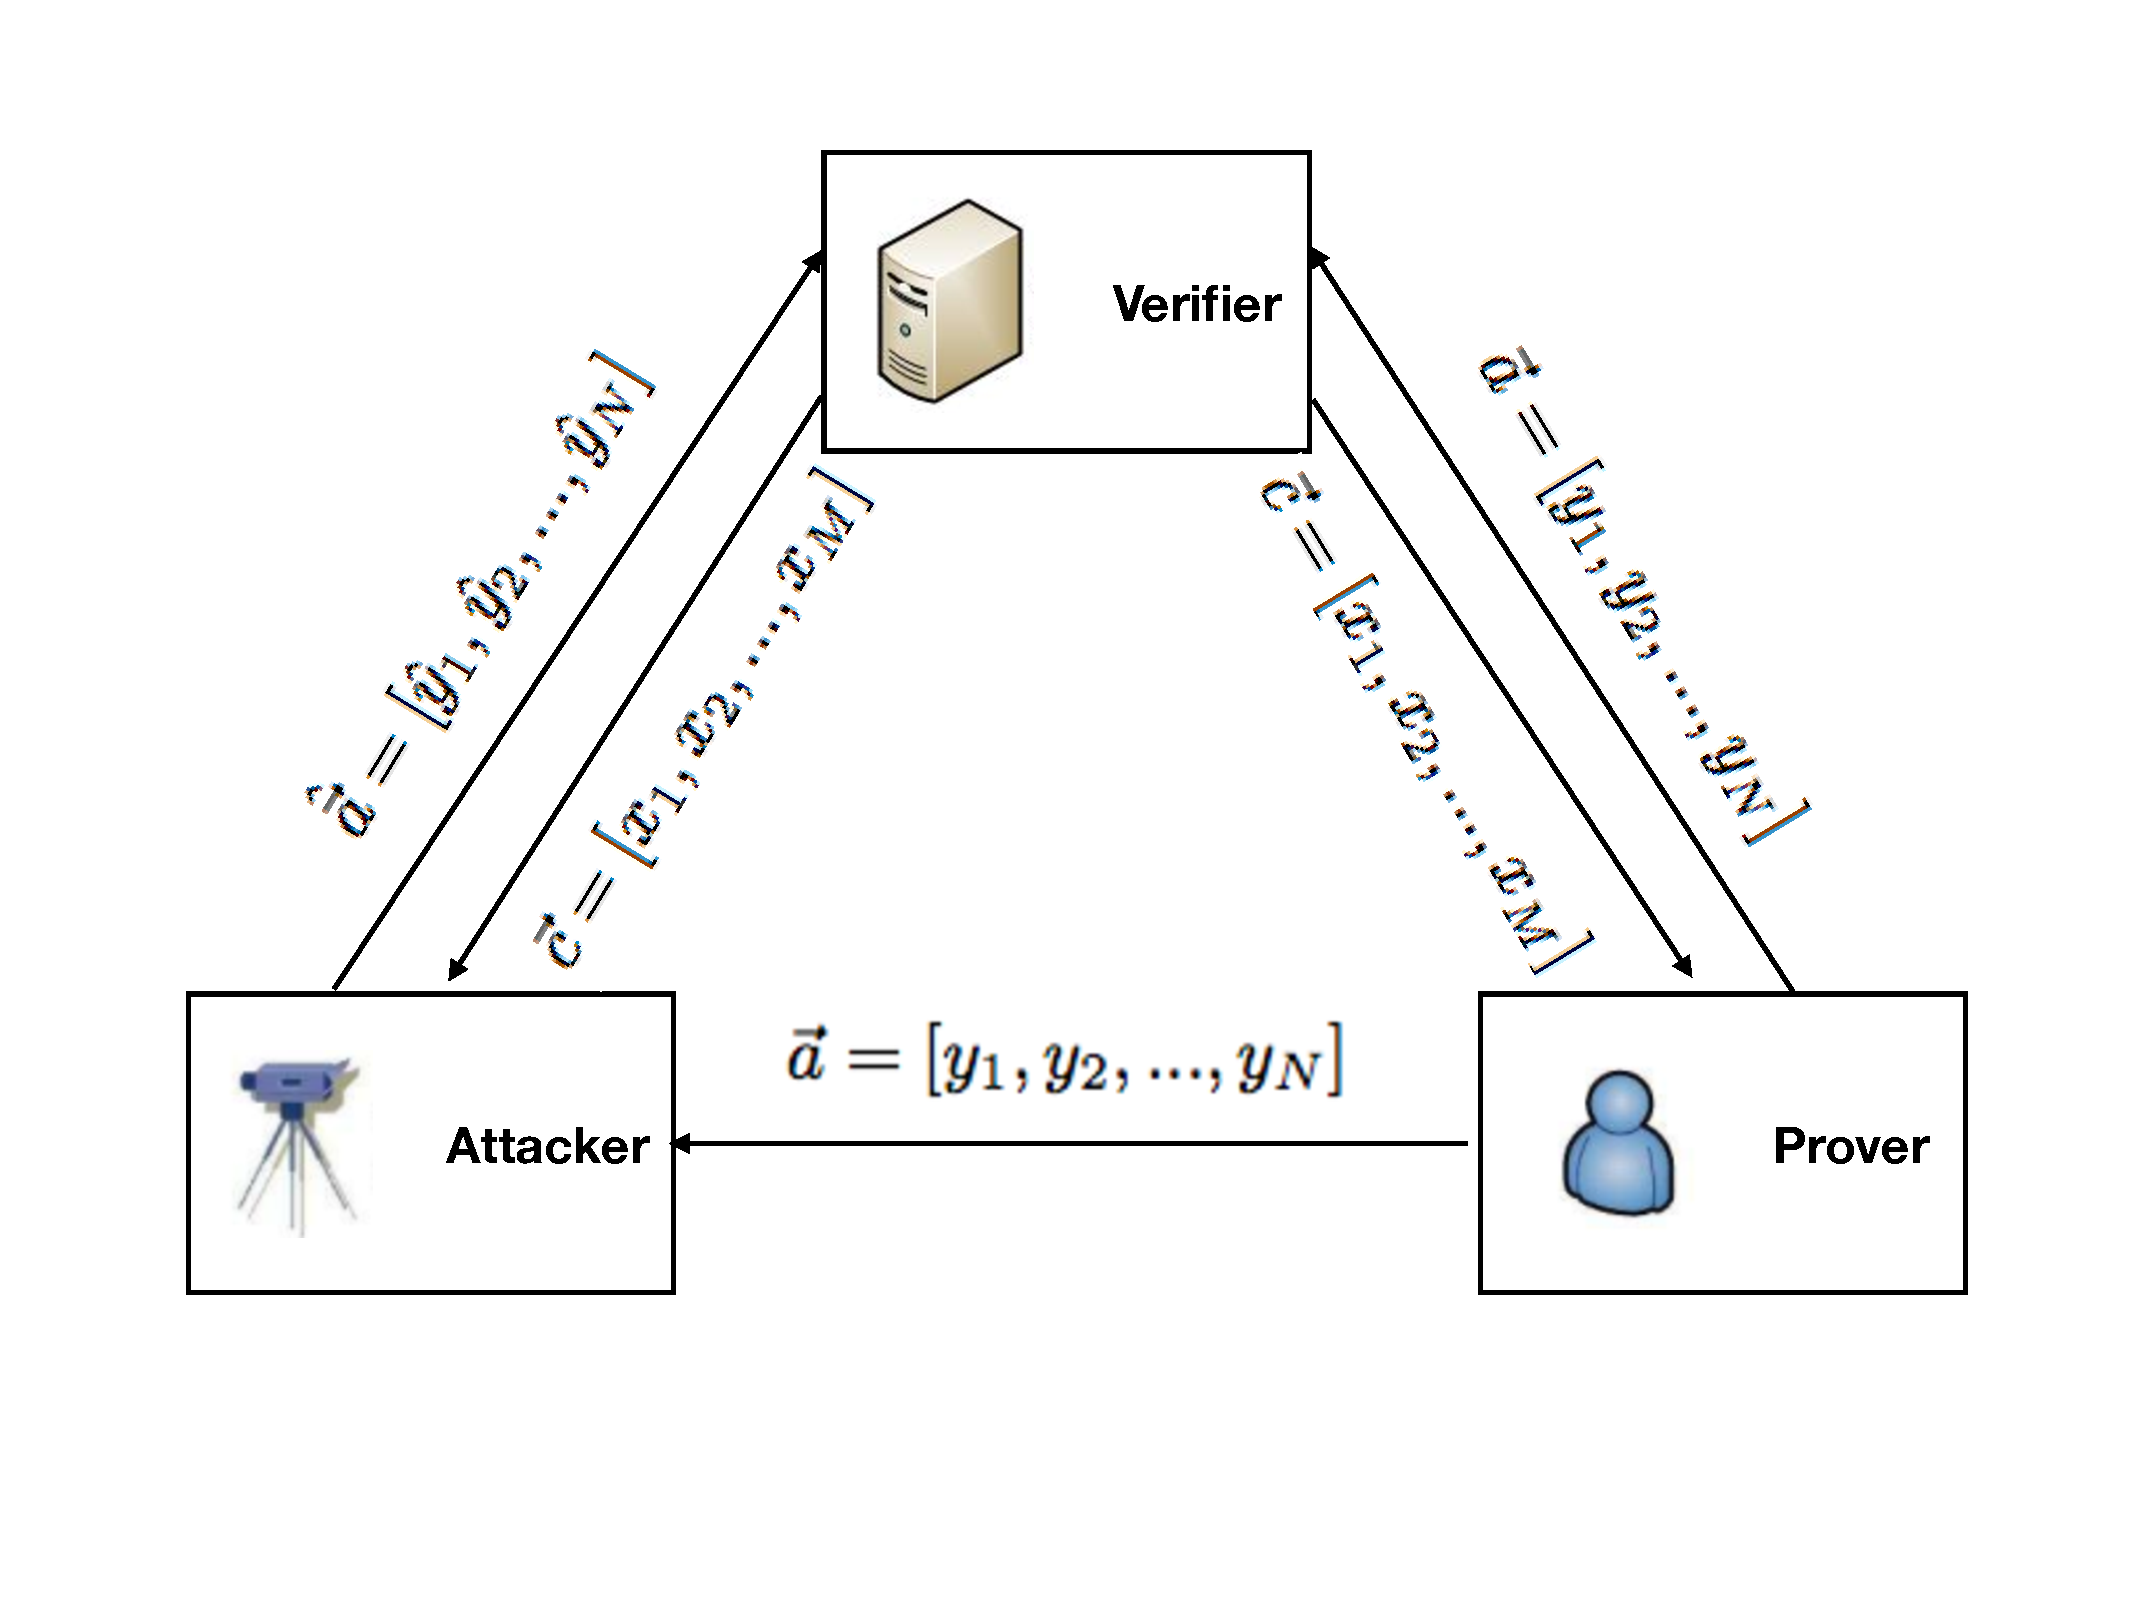
\includegraphics[width=8.5cm]{architecture.pdf}
    \caption{The architecture of graphical password systems}
    \label{fig:architecture}
  \end{figure}
  As shown in Figure \ref{fig:architecture}, a graphical password system is constituted with a verifier (computers), 
  $K$ provers (human users)and a attacker. 
  
  The verifier is responsible for the verifications of provers. It maintains $[p_1, p_2,...,p_{K}]$, 
  which $p_i$ is the authentication password of prover $i$. In the authentication process, it generates $K$ 
  authentication challenges $[\vec{c}_1, \vec{c}_2,...,\vec{c}_{K}]$ for each prover and collects relative replies 
  $[\vec{a}_1,\vec{a}_2,...,\vec{a}_{K}]$ from each prover. The verifier distinguishs true provers $\mathbb{T}$ 
  from attackers, where $\mathbb{T} = \{i|p_i(\vec{c}_i) = \vec{a}_i\}$.

  % The verifier has three main functions. First, the verifier generates a specific authentication challenge $c$ for 
  % a prover and collects a reply $a$ from the prover. Then, it memorizes passwords of all provers. 
  % Besides, the verifier is responsible for the verification of provers:
  % \begin{equation}
  %   Verifier(a)=
  % \left\{
  %  \begin{aligned}
  %  1, \quad p(c) = a \\
  %  0, \quad p(c) \neq a
  %  \end{aligned}
  %  \right.
  %  , \quad a \in \mathbb{A}
  % \end{equation}
  For prover $i$, it gets an authentication challenge $\vec{c}_i$ from the verifier and replied with an 
  authentication answer $\vec{a}_i = p_i(\vec{c}_i)$. Prover $i$ can login only if $i \in \mathbb{T}$. 
  
  The attacker hides in the system, records successive challenge and answer pairs $(c, a)$ and trains 
  NN enabled attack models for different provers. The result of an attack is determined by Equation \ref{equa:attacker}, 
  and $Attack(\vec{c}_i,\vec{a}_i)=1$ will be viewed as a successful attack on prover $i$.
  \begin{equation}
    Attack(\vec{c}, \vec{a})=
  \left\{
   \begin{aligned}
   1, \quad NN(\vec{c}) = \vec{a} \\
   0, \quad NN(\vec{c}) \neq \vec{a}
   \end{aligned}
   \right.
  \label{equa:attacker}
  \end{equation}
  
  
  \section{Design of an Attack Model}
  \label{sec:design}
  In this section, we described the design of an attack model. We started by explaining the training 
  methodology. Then we described the hierarchy of the NN model used in the attack model and enabled it 
  to support different graphical password systems.
  
  The first step for the attack model is to generate a training phase. Ideally, training data would be collected with actual 
  shoulder-surfing attacks. However, this approach is inefficient, as the training algorithm must wait until an attack 
  finished and relevant information was recorded into the training phase. To accelerate the process, we train 
  the attack model in a simple simulation environment that faithfully models the authentication process. The 
  attack model's simulator maintains a verifier and a prover, which generated authentication challenges and 
  relevant answers successively.
  
  The hierarchy of attack models is as followed. The input is a $M$-dimensional vector 
  $\vec c = [x_1, x_2,...,x_M]$, which a simulation of an authentication challenge. The output is simply a 
  predicted $N$-bit answer with respect to the authentication challenge. The input layer is simply $M$ units, 
  i.e. one for each bit of an authentication challenge. The hierarchy of hidden layers is optional for 
  attackers. The output layers differed between different passwords. For the prediction of the $i$-bit authentication 
  answer, if $S_y^i$ is known by attackers in advance we will use a $|S_y^i|$-way softmax as predict the $i$-bit 
  of the authentication answer. Otherwise the softmax layer will be replaced by a regression layer. The $i$-bit 
  authentication answer can be predicted as:
  \begin{equation}
    \begin{gathered}
    a_i = (1-known(S_y^i))(\sum_{i=1}^H w_ix_i) \\
    + known(S_y^i)(\mathop{\arg\max}_{k \in S_y^i}\frac{exp(x_k)}{\sum_{j=1}^{S_y^i}exp(x_j)})
    \end{gathered}
  \end{equation}
  where $H$ is the size of the last hidden layer, $x_i$ is the output of the $i$-th unit in the last hidden layer. 
  $known(S_y^i) = 1$ when $S_y^i$ is known in advance, otherwise $known(S_y^i) = 0$.
  
  The NN enabled attack models only focus on the high precision, which means attackers could pass the authentication 
  with a higher probability. The characteristic of NN enabled attack model distinguish it from traditional 
  NN models, as the latter pay equal attention to precision and recall rate.
  
  With the NN enabled attack model, we could quantify passwords strength against shoulder-surfing attacks 
  from attackers' view, since the difficulty of NN training indirectly reflects password strength against 
  shoulder-surfing attacks.  Given training set $R_{train}$ and test set $R_{test}$, we defined an indicator 
  to quantify the strength of password system $pass$ against shoulder-surfing attacks:
  \begin{equation}
    \begin{gathered}
    Strength_{pass|l} = \mathop{\min}\ \ |R_{train}| \\
    s.t.\ 
    \forall (c,a) \in R_{test}, P(Attack(c,a)=1|R_{train}) \geq l
    \end{gathered}
  \label{equa:indictor}
  \end{equation}
  
  The indicator $Strength_{pass|l}$ is highly influenced by the information expressivity of NN models. Therefore, for the 
  rationality of the comparisons of password strength, the information expressivities of all NN models should 
  be similar when $Strength_{pass|l}$ is used to quantify multiple password systems at the same time.
  \section{Evaluation}
  \label{sec:evaluation}
  In this section, we first introduce two categories of advanced graphical password systems, and present 
  information about our dataset and model architectures. We then make two experiments and study the 
  rationality of our indicator $Strength_{pass|l}$ and the influence of NN models' expressivity. The project 
  can be downloaded in Github. See \cite{gys} for detail.
  \subsection{Experiment setup}
  \textbf{Categories of Advanced graphical password systems:}
  Advanced graphical passwords can be divided into two main categories based on recall and recognition. 
  Recognition-based systems generally ask users to memorize a portfolio of images during password creation and 
  then recognize their images from among decoys \cite{DBLP:journals/csur/BiddleCO12}. 
  PassFaces \cite{Passfaces} is the canonical example of recognition-based graphical passwords. PassFaces has a 
  pool of $F$ human face pictures, where users pre-select $A$ human faces. During login, a panel of $B$ 
  candidate faces is presented. Users must select the face belonging to their set from among decoys. $C$ such 
  rounds are repeated with different panels (generally $C < A$). 
  
  Recall-based graphical password systems are referred to as drawmetric systems \cite{DBLP:journals/ijmms/AngeliCJR05}. 
  In the recall-based systems, users recall the pattern they selected before and calculate an authentication 
  answer based on the pattern. GrIDsure \cite{Brostoff2010Evaluating} is a kind of recall-based graphical password system, which displays digits in a $D \times D$ grid. 
  Users select and memorize a pattern consisting of an ordered subset of $E$ grid squares in advance. On 
  subsequent logins, digits are randomly displayed within the grid squares and users enter the sum of digits 
  within their memorized pattern.
  
  \textbf{Setup:}We made experiments on $6$-bit PIN, indefinite length ($\leq 12$) 
  text password, PassFaces and GrIDsure. $6$-bit PIN has been 
  widely used in ATM and online payment environments, and indefinite length text passwords are applied in social 
  applications, like Facebook and Twitter. These two kinds of password systems are on behalf of traditional 
  graphical passwords. Passfaces and GrIDsure are two canonical examples of advanced graphical passwords. In the 
  experiments, $A = 5, B = 9, C = 1, D = 3, E = 4, F=100$.
  
  We use Keras to construct attack models for these four graphical passwords. Keras is a high-level neural networks 
  API, developed with a focus on enabling fast experimentation \cite{chollet2015keras}. We utilize a sequential model in our experiment. 
  There are two hidden layers for all attack models, and each layer has an identical number of hidden units. Identical hidden layers ensure 
  that the four NN models have similar information expressivity. The number of units in the input and output 
  layers is determined by the size of authentication challenges and answers of different password systems, 
  which makes little influence on the information expressivity. In the training process, we train each NN model with 
  10 different training sets and compute the average precision. We use RMSProp as the optimizer.
  
  \subsection{Experiment results}
  In the first experiment, we try to verify the rationality of our indicator $Strength_{pass|l}$. All the NN 
  models in this experiment have two hidden layers, each layer has $32$ hidden units. We record the precision 
  rate of four attack models when giving different sizes of training sets. 
  \begin{figure}[htb]
    \centering
    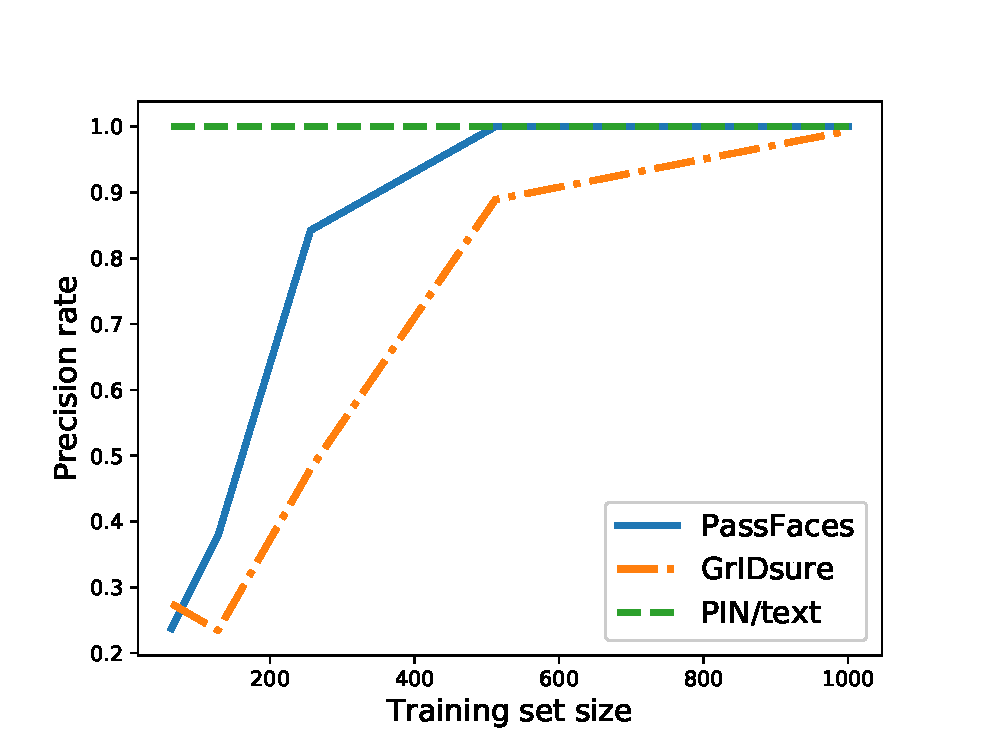
\includegraphics[width=8.5cm]{line.eps}
    \caption{The precision of different graphical passwords when given different training sets}
    \label{fig:results}
  \end{figure}
  
  The result is shown in Figure \ref{fig:results}. To achieve a more than $90\%$ precision, the NN models for 
  PIN/text need really small training set, the NN model for PassFaces need $256$ pieces of training data, and 
  about $500$ pieces of training data are needed for GrIDsure. The result illustrates that GrIDsure and PassFaces 
  have greater capabilities than PIN/text passwords to protect from shoulder-surfing attacks, and GrIDsure 
  is even better than PassFaces. The experiment result is consistent with the theoretical analysis. The challenge space $\mathbb{C}$
  and answer space $\mathbb{A}$ of PIN and text passwords are zero-dimension, so the authentication passwords in these systems 
  are constant functions, which are vulnerable to shoulder-surfing attacks. For PassFaces, 
  $|\mathbb{C}| = \binom{F}{B}, |\mathbb{A}| = \binom{A}{C}$, and the authentication password is a injective function, which 
  is harder for NN models to crack. GrIDsure has an even larger challenge space and answer space, so it is least 
  vulnerable to shoulder-surfing attacks.
  
  The result also reveals the vulnerability of PIN and text passwords against shoulder-surfing attacks. Nowadays, 
  these two traditional password systems are broadly implemented in mobile devices, which meet with high security 
  risks. This is what we think the Internet industry really has to pay attention.
  
  In the second experiment, we build up several NN models with different information expressivities and study 
  their influence on the indicator $Strength_{pass|l}$.
  \begin{figure}[htb]
    \centering
    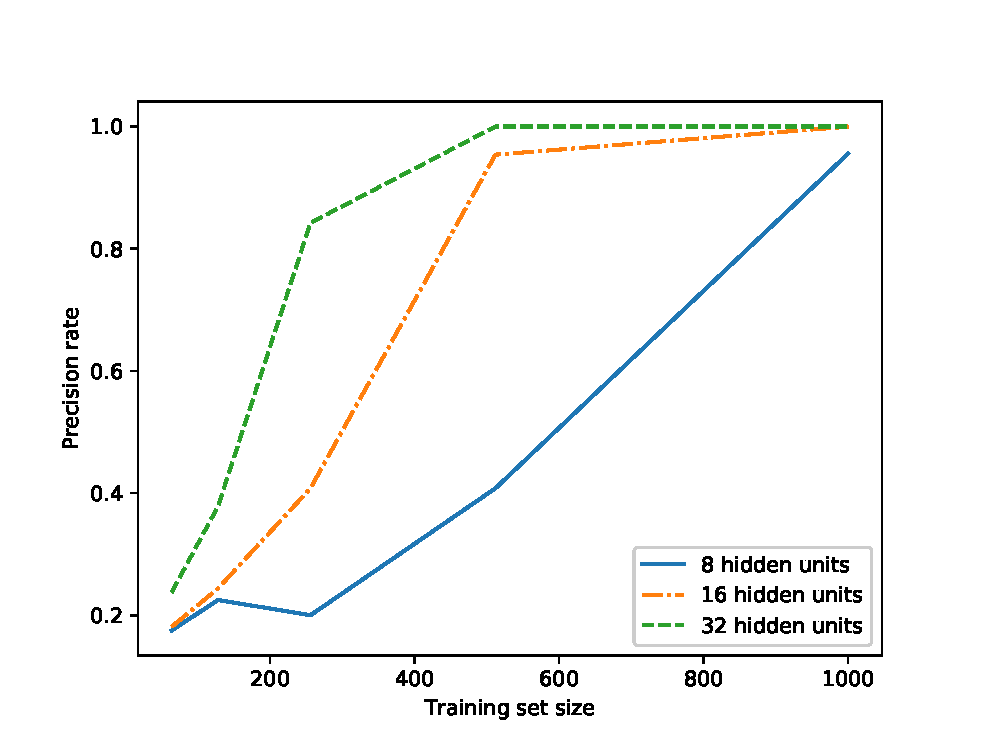
\includegraphics[width=8.5cm]{passfaces.eps}
    \caption{The influence of information expressivity on PassFaces's NN model. The precision is really 
    low when there are $8$ hidden units in each hidden layer.}
    \label{fig:results2}
  \end{figure}
  % \begin{figure}[htb]
  %   \begin{minipage}[b]{.48\linewidth}
  %   \centering
  %   \centerline{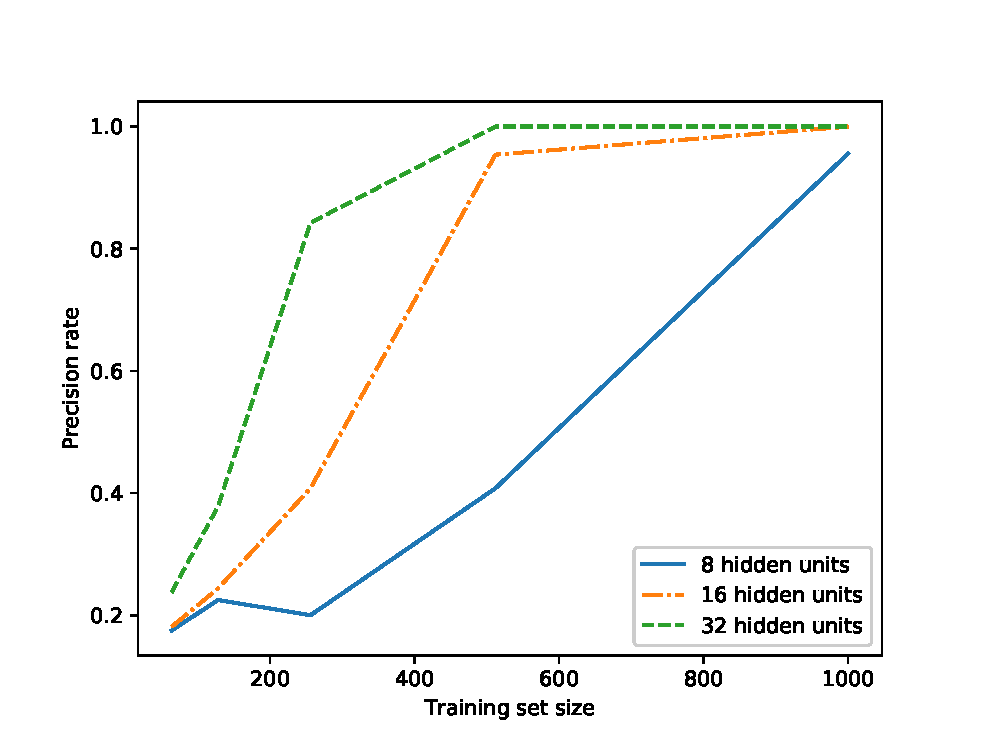
\includegraphics[width=4.0cm]{passfaces.eps}}
  % %  \vspace{1.5cm}
  %   \centerline{PassFaces}\medskip
  % \end{minipage}
  % \hfill
  % \begin{minipage}[b]{0.48\linewidth}
  %   \centering
  %   \centerline{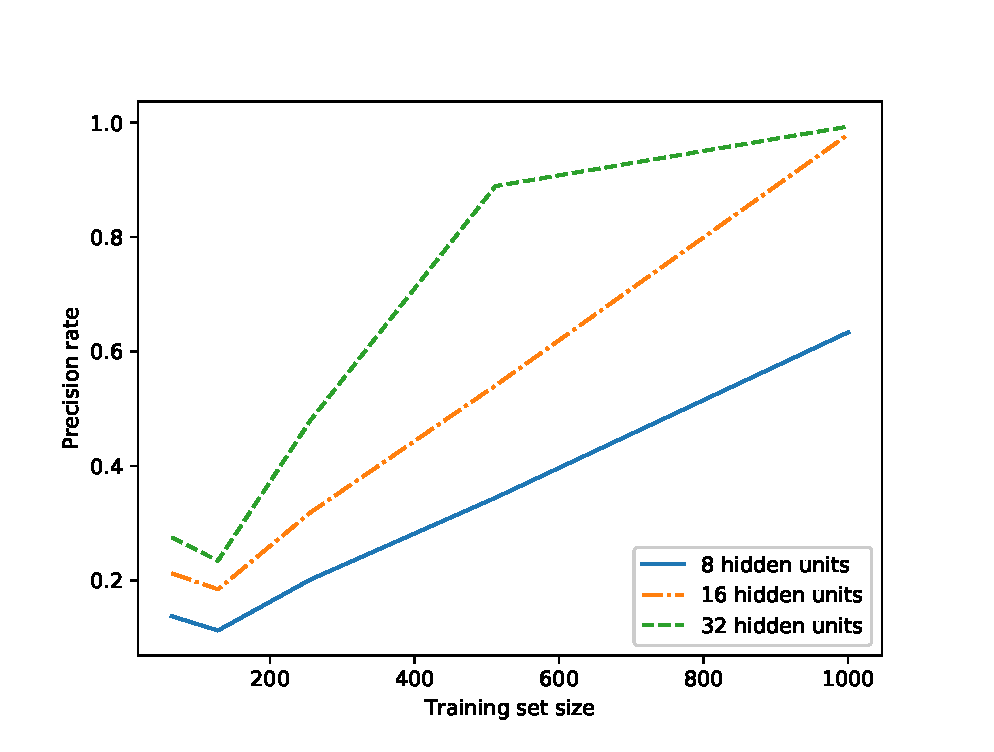
\includegraphics[width=4.0cm]{gridsure.eps}}
  % %  \vspace{1.5cm}
  %   \centerline{GrIDsure}\medskip
  % \end{minipage}
  %   \label{fig:results2}
  % \end{figure}
  
  Figure \ref{fig:results2} shows the experiment results on PassFaces and GrIDsure. When there is $8$ hidden 
  units in each hidden layer, $Strength_{PassFaces|0.9}$ approaches $1000$. However, $Strength_{PassFaces|0.9}$ halves 
  when the number of hidden units increases to $32$. We do not display the result on GrIDsure due to space 
  limitations, and it shows great similarities with PassFaces on the experiment result. The attack model can not 
  get a $90\%$ accuracy even with $1000$ pieces of training data when there are $8$ hidden units each layer.
  
  The second experiment shows that information expressivities of NN models seriously affect $Strength_{pass|l}$. 
  The result is significant both for attackers and researchers. For attackers, the shoulder-surfing attack will be 
  more efficient when using state-of-the-art NN models. And for researchers, the architecture of the NN model should 
  be mentioned when quantifying a password system. Otherwise the indicator will be meaningless.
  
  \section{Conclusion}
  \label{sec:conclusion}
  In this paper, we proposed a standardized method to quantify graphical password strength against NN enabled 
  shoulder-surfing attacks. We also revised some basic definitions and presented a NN-enabled attack model. 
  We then made experiments on four representative graphical password systems and studied the rationality of 
  our indicator $Strength_{pass|l}$ and the influence of NN's information expressivity. In the experiments, 
  we found traditional PIN and text passwords encountered serious security risks with shoulder-surfing attacks. 
  
  A possible direction for future work is adapting the indicator and taking time complexity into consideration.
  
  % Below is an example of how to insert images. Delete the ``\vspace'' line,
  % uncomment the preceding line ``\centerline...'' and replace ``imageX.ps''
  % with a suitable PostScript file name.
  % -------------------------------------------------------------------------
  % \begin{figure}[htb]
  
  % \begin{minipage}[b]{1.0\linewidth}
  %   \centering
  %   \centerline{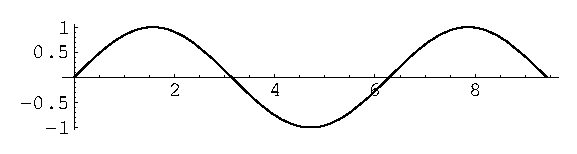
\includegraphics[width=8.5cm]{image1}}
  % %  \vspace{2.0cm}
  %   \centerline{(a) Result 1}\medskip
  % \end{minipage}
  % %
  % \begin{minipage}[b]{.48\linewidth}
  %   \centering
  %   \centerline{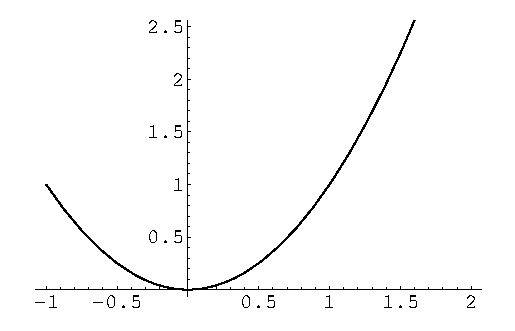
\includegraphics[width=4.0cm]{image3}}
  % %  \vspace{1.5cm}
  %   \centerline{(b) Results 3}\medskip
  % \end{minipage}
  % \hfill
  % \begin{minipage}[b]{0.48\linewidth}
  %   \centering
  %   \centerline{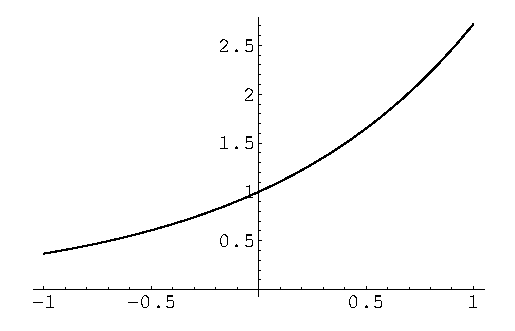
\includegraphics[width=4.0cm]{image4}}
  % %  \vspace{1.5cm}
  %   \centerline{(c) Result 4}\medskip
  % \end{minipage}
  % %
  % \caption{Example of placing a figure with experimental results.}
  % \label{fig:res}
  % %
  % \end{figure}
  
  
  % To start a new column (but not a new page) and help balance the last-page
  % column length use \vfill\pagebreak.
  % -------------------------------------------------------------------------
  %\vfill
  %\pagebreak
  
  
  \vfill\pagebreak
  
  
  % References should be produced using the bibtex program from suitable
  % BiBTeX files (here: strings, refs, manuals). The IEEEbib.bst bibliography
  % style file from IEEE produces unsorted bibliography list.
  % -------------------------------------------------------------------------
  \bibliographystyle{IEEEbib}
  \bibliography{refs}
  
  \end{document}
  